% ******************************************************** %
%              TEMPLATE DE INFORME ORGA2 v0.1              %
% ******************************************************** %
% ******************************************************** %
%                                                          %
% ALGUNOS PAQUETES REQUERIDOS (EN UBUNTU):                 %
% ========================================
%                                                          %
% texlive-latex-base                                       %
% texlive-latex-recommended                                %
% texlive-fonts-recommended                                %
% texlive-latex-extra?                                     %
% texlive-lang-spanish (en ubuntu 13.10)                   %
% ******************************************************** %


\documentclass[a4paper]{article}
\usepackage[spanish]{babel}
\usepackage[utf8]{inputenc}
\usepackage{charter}   % tipografia
\usepackage{tipa}
\usepackage{graphicx}
%\usepackage{makeidx}
\usepackage{paralist} %itemize inline

\usepackage{float}
\usepackage{amsmath, amsthm, amssymb}
%\usepackage{amsfonts}
%\usepackage{sectsty}
%\usepackage{charter}
%\usepackage{wrapfig}
%\usepackage{listings}
%\lstset{language=C}

% \setcounter{secnumdepth}{2}
\usepackage{underscore}
\usepackage{caratula}
\usepackage{url}
\usepackage{caption, subcaption}
\usepackage{placeins}

% ********************************************************* %
% ~~~~~~~~              Code snippets             ~~~~~~~~~ %
% ********************************************************* %

\usepackage{color} % para snipets de codigo coloreados
\usepackage{fancybox}  % para el sbox de los snipets de codigo

\definecolor{litegrey}{gray}{0.94}

\newenvironment{codesnippet}{%
	\begin{Sbox}\begin{minipage}{\textwidth}\sffamily\small}%
	{\end{minipage}\end{Sbox}%
		\begin{center}%
		\vspace{-0.4cm}\colorbox{litegrey}{\TheSbox}\end{center}\vspace{0.3cm}}



% ********************************************************* %
% ~~~~~~~~         Formato de las páginas         ~~~~~~~~~ %
% ********************************************************* %

\usepackage{fancyhdr}
\pagestyle{fancy}

%\renewcommand{\chaptermark}[1]{\markboth{#1}{}}
\renewcommand{\sectionmark}[1]{\markright{\thesection\ - #1}}

\fancyhf{}

\fancyhead[LO]{Sección \rightmark} % \thesection\ 
\fancyfoot[LO]{\small{Nombre Apellido, Nombre Apellido, Nombre Apellido}}
\fancyfoot[RO]{\thepage}
\renewcommand{\headrulewidth}{0.5pt}
\renewcommand{\footrulewidth}{0.5pt}
\setlength{\hoffset}{-0.8in}
\setlength{\textwidth}{16cm}
%\setlength{\hoffset}{-1.1cm}
%\setlength{\textwidth}{16cm}
\setlength{\headsep}{0.5cm}
\setlength{\textheight}{25cm}
\setlength{\voffset}{-0.7in}
\setlength{\headwidth}{\textwidth}
\setlength{\headheight}{13.1pt}

\renewcommand{\baselinestretch}{1.1}  % line spacing

% ******************************************************** %


\begin{document}


\thispagestyle{empty}
\materia{Organización del Computador II}
\submateria{Primer Cuatrimestre de 2019}
\titulo{Trabajo Práctico II}
\subtitulo{Filtros en SIMD}
\integrante{Sotomayor Marco}{731/14}{marco.soto1995@gmail.com}
\integrante{Tejera Walter}{362/15}{wtejerac@gmail.com}

\maketitle
\newpage

\thispagestyle{empty}
\vfill


\thispagestyle{empty}
\vspace{3cm}
\tableofcontents
\newpage


%\normalsize
\newpage

\section{Introducción}

SIMD (single instruction, multiple data) es una arquitectura de computaci\'on centrada en el procesamiento simultaneo de una operaci\'on sobre varios datos mediante una \'unica isntrucci\'on. Tal t\'ecnica suele ser aplicada para trabajar de manera eficiente sobre vectores y matrices de datos. \par
El objetivo de este trabajo pr\'actico es consolidar los conocimientos adquiridos en las clases sobre SIMD. Utilizando esta arquitectura implementaremos distintos algoritmos en ASM creando filtros sobre imágenes para luego comparar su rendimiento contra su implementación en C.


\section{Desarrrollo}

\begin{figure}
  \begin{center}
	
\includegraphics[scale=0.66]{img/logouba.jpg}
	\label{nombreparareferenciar}
  \end{center}
\end{figure}

\subsection{Imagen Fantasma}

\subsubsection{Descripci\'on}

\paragraph{} Este filtro consiste en generar una imagen fantasma sobre la original, para ello se utiliza la misma imagen original al doble de tamaño y en escala de grises. Ademas se generara a partir de un punto cuyas coordenadas nos dan por parametro.

\subsubsection{Implementaci\'on}

\paragraph{} En esta implementaci\'on se realizan dos recorridos diferentes por cada iteraci\'on sobre la matriz $src$: 
\begin{itemize}
	\item Uno de los recorridos es similar al implementado en C, es decir recorriendo todos los pixeles de cada fila. Con la principal diferencia de que se levantan 4 pixeles en vez de 1.
	\item En nuestra implementaci\'on no se calcula $ii$ ni $jj$, en cambio existe un segundo recorrido que levanta los pixeles correspondientes a estos indices.
\end{itemize}

\paragraph{Recorrido de $ii$ y $jj$:} 
\begin{center}
	Sabemos que $ii = i/2 + offset_x$ , \, $jj = j/2 + offset_y$ representando $"/"$ la divisi\'on entera. Fijando el $offset_y$ en 0 veamos como cambia $jj$ a partir de una sucesi\'on de valores para $j$:
	
	\begin{align*}
		j &= [0, 1, 2, 3, 4, 5, 6, 7, 8, 9]\\
		jj &= [0, 0, 1, 1, 2, 2, 3, 3, 4, 4]
	\end{align*}    
	
	\paragraph{} El valor de $jj$ para los $j$ impares es el mismo que para el par menor y mas cercano a ese $j$ impar, ya que el operador $"/"$ descarta el resto y devuelve solo el cociente es decir: $j = 2*q \, \wedge \, j+1 = 2*q + r \Rightarrow j/2 = q$ \, y \, $(j+1)/2 = q$. Podemos usar esta informaci\'on para afirmar que si $j = 2 * q \Rightarrow jj(j) == jj(j+1)$ (notar que en el calculo de $jj$, $offset_x$ es siempre la misma constante sumada, no cambia la igualdad).
	
	\paragraph{} Esto lo aprovechamos para no calcular $ii$ ni $jj$ en cada iteraci\'on, ya que $i, j$ empiezan en $0 \Rightarrow ii = offset_y, jj=offset_x$. Luego basta con incrementar en 1 a $ii$ o $jj$ por cada 2 incrementos de $i$ y $j$ respectivamente (en nuestro caso los incrementos son de a 2 para $jj$ y 4 para $j$ ya que se procesan 4 pixeles).
\end{center}


\paragraph{}Para calcular $B$, utilizamos una mascara que reordena las componentes de los 2 pixeles $m[ii][jj]$ y $m[ii][jj+1]$ de la siguiente manera: $blue, green, red, green$. Este nuevo orden permite que realicemos una suma horizontal, sin embargo no existe suma horizontal de a Byte, por lo que adem\'as extendemos con 0 cada byte usando la misma mascara.  

\begin{align*}
	xmm &= [\, \, \, \, * \, \, \, \, \, ,\, \, \, \, \, * \, \, \, \, \, ,\, \, \, \, * \, \, \, \, \, ,\, \, \, \, * \, \, \, \, \, ,\, \, \, \, * \, \, \, \, \, \, ,\, \, \, \, * \, \, \, \, \, ,\, \, \, \, * \, \, \, \, \, ,\, \, \, \, * \, \, \, \, \, \, , \, \, \, \,  A_1 \, , \, \, \, \, R_1 \, , \, \, \, \, G_1 \, , \, \, \, \, B_1 \, , \, \, \, \, A_0 \, , \, \, \, \, R_0 \, , \, \, \, \, G_0 \, , \, \, \, \, B_0 \, \,]\\
	mascara &= [0x80, 0x05, 0x80, 0x06, 0x80, 0x05, 0x80, 0x04, 0x80, 0x01, 0x80, 0x02, 0x80, 0x01, 0x80, 0x00] \\
\end{align*}
	\hrule
\begin{align*}
	pshufb &= [G_1, R_1, G_1, B_1, G_0, R_0, G_0, B_0] \leftarrow \text{en words}
\end{align*} 

\paragraph{}Una vez ordenadas las componentes se ejecutan 2 sumas horizontales para generar $B_0$ y $B_1$ en los dos words menos significativos del registro. Separamos los $B$ en registros diferentes ($R_{b0}$, $R_{b1}$) y desempaquetamos a doublewords cada uno, adem\'as replicamos cada $B$ en los 4 doubleword en su respectivo registro. Luego los convertimos en floats para dividirlos por 8 (b/4/2 == b/8).

\paragraph{} Para procesar los pixeles, realizamos los siguiente pasos:

\begin{itemize}
	\item Se mueven los 4 pixeles a 4 registros diferentes: $R_{px0}$, $R_{px1}$, $R_{px2}$ y $R_{px3}$.
	\item En cada registro se realizan las conversiones necesarias para pasar de bytes a words y de words a doublewords para el pixel que le corresponda.
	\item Convertimos las componentes de cada registro a floats.
	\item Realizamos multiplicaciones vectoriales entre una constante con 4 datos de tipo float con valor 0,9 y cada uno de los $R_{px}$.
	\item Sumamos $R_{px0}$, $R_{px1}$ con $R_{b0}$ y $R_{px2}$, $R_{px3}$ con $R_{b1}$.
\end{itemize}

Con esto tenemos nuestros 4 pixeles procesados. Por \'ultimo queda realizar 4 conversiones de float con truncamiento a doubleword en $R_{px0}$, $R_{px1}$, $R_{px2}$ y $R_{px3}$. Desempaquetamos (haciendo las conversiones intermedias) cada registro en 1 solo que junte los 4 pixeles procesados y lo guardamos en el destino.

\paragraph{Comentarios sobre el signado en operaciones:} Algunas conversiones u operaciones no existen para n\'umeros sin signo, esto puede generar problemas si lo n\'umeros sin signo sobre los que se quiere operar son tan grandes que su representaci\'on binaria tiene el bit mas significativo en 1, pues en su interpretaci\'on signada serian negativos.
\paragraph{}Los n\'umeros mas grande sobre los que trabajamos son $B$ y $componente(px) * 0,9 + B/2$. Si todas las componentes de $m[ii][jj]$ valen 255 $\Rightarrow B = 4*255/4 = 255$. Luego $componente(px) * 0,9 + B/2 \simeq  230 + 126 \simeq 356$. Como todas las operaciones son realizadas luego de convertir los datos al menos a words tenemos los suficientes bits para representar $356$ sin usar el bit mas significativo.

\subsection{Color Bordes}
\subsubsection{Descripci\'on}

\paragraph{} Color bordes modifica cada pixel operando mediante restas sobre los 8 pixeles que lo rodean, generando valores pequeños y similares para cada componente si los 8 pixeles tenían un color parecido entre ellos y variando estos valores en caso contrario. Esto genera diferentes componentes conexas con colores oscuros separadas por bordes de colores variables y claros. Adem\'as agrega un marco blanco de 1 pixel.  

\subsubsection{Desarrollo}

\paragraph{} La matriz se recorre de manera similar a la implementaci\'on en C, pero en cada iteraci\'on se modifican 2 pixeles. Utilizamos las herramientas de SIMD para levantar 3 filas ($i-1$, $i$ y $i+1$) de 4 pixeles, re ordenar los datos y luego operar. Nos referiremos a cada una de estas filas con mediante los nombres $R_{i-1}$, $R_i$ y $R_{i+1}$. Llamaremos $px0$, $px1$, $px2$ y $px3$ a los pixeles de cada fila. Modificaremos $px1$ y $px2$ de $R_i$.

\paragraph{ii:} Con el objetivo de realizar $m[ii][j-1] - m[ii][j+1]$ mediante restas horizontales armamos 2 mascaras, una para procesar los datos de $px1$ y otra para $px2$. Esta mascara adem\'as extiende los datos de byte a words con ceros. A continuaci\'on mostraremos la mascara para procesar las operaciones de $px1$ y $px2$.
 


\begin{align*}
	R_i &= [\, \, \, \, A_3 \, ,\, \, \, \, \, R_3 ,\, \, \, \, G_3 \, ,\, \, \, \, B_3 \, ,\, \, \, \, A_2 \, ,\, \, \, \, R_2 \, ,\, \, \, \, G_2 \, ,\, \, \, \, B_2 \, , \, \, \, \,  A_1 \, \, , \, \, \, \, R_1 \, , \, \, \, \, G_1 \, , \, \, \, \, B_1 \, , \, \, \, \, A_0 \, \, , \, \, \, \, R_0 \, , \, \, \, \, G_0 \, , \, \, \, \, B_0 \, \,]\\
	indice &= [0x0f, 0x0e, 0x0d, 0x0c, 0x0b, 0x0a, 0x09, 0x08, 0x07, 0x06, 0x05, 0x04, 0x03, 0x02, 0x01, 0x00]\\
	mascara_{px1} &= [0x80, 0x80, 0x80, 0x80, 0x80, 0x0A, 0x80, 0x02, 0x80, 0x09, 0x80, 0x01, 0x80, 0x08, 0x80, 0x00] 
\end{align*}
\hrule
\begin{align*}
	pshufb_{px1} &= [0, 0, R_2, R_0, G_2, G_0, B_2, B_0] \leftarrow \text{en words}
\end{align*} 


\begin{align*}
	R_i &= [\, \, \, \, A_3 \, ,\, \, \, \, \, R_3 ,\, \, \, \, G_3 \, ,\, \, \, \, B_3 \, ,\, \, \, \, A_2 \, ,\, \, \, \, R_2 \, ,\, \, \, \, G_2 \, ,\, \, \, \, B_2 \, , \, \, \, \,  A_1 \, \, , \, \, \, \, R_1 \, , \, \, \, \, G_1 \, , \, \, \, \, B_1 \, , \, \, \, \, A_0 \, \, , \, \, \, \, R_0 \, , \, \, \, \, G_0 \, , \, \, \, \, B_0 \, \,]\\
	indice &= [0x0f, 0x0e, 0x0d, 0x0c, 0x0b, 0x0a, 0x09, 0x08, 0x07, 0x06, 0x05, 0x04, 0x03, 0x02, 0x01, 0x00]\\
	mascara_{px2} &= [0x80, 0x80, 0x80, 0x80, 0x80, 0x0E, 0x80, 0x06, 0x80, 0x0D, 0x80, 0x05, 0x80, 0x0C, 0x80, 0x04] 
\end{align*}
\hrule
\begin{align*}
	pshufb_{px2} &= [0, 0, R_3, R_1, G_3, G_1, B_3, B_1] \leftarrow \text{en words}
\end{align*} 

\paragraph{} Copiamos $R_{i-1}$, $R_i$ y $R_{i+1}$ en 3 registros, uno para cada uno, luego a los 3 originales aplicamos una mascara y a las 3 copias aplicamos la mascara restante. Teniendo los datos acomodados en 6 registros los siguientes pasos son directos y simples. Primero realizamos una resta horizontal en cada uno de ellos consiguiendo $m[ii][j-1] - m[ii][j+1]$ de cada componente, luego aplicamos el valor absoluto y acumulamos los valores de cada componente.

\paragraph{jj :}En este caso primero operamos y luego reordenamos los datos. Esta vez nuestro iterador es $jj$ y se mueve por $j$ mientras que opera entre las filas $i-1$ e $i+1$. Queremos calcular $m[i-1][jj] - m[i+1][jj]$ para cada componente.

\begin{itemize}
	\item Desempaquetamos $R_{i-1}$ y $R_{i+1}$ a words.
	\item Restamos $R_{i-1}$ y $R_{i+1}$ desempaquetados.
	\item Aplicamos valor absoluto a los resultados
	\item A partir de este punto tenemos 2 registros $R_1$ y $R_2$. $R_1$ contiene las restas en words de los componentes de $j$ y $j-1$, mientras $R_2$ contiene las restas de $j+2$ y $j+1$.
	\item Para acumular estos resultados utilizo 1 registro intermedio para cada uno. Paso $R_1$ a $R_3$ y shifteo los resultados $j$ a la parte mas baja de $R_3$. Ahora el primer word de $R_1$, $R_2$ y $R_3$ contienen los resultados de $j-1$, $j+1$ y $j$ respectivamente.
	\item Sumamos los 3 registros y obtenemos las acumulaciones $jj$ de las operaciones entre componentes para $px1$. Haciendo un proceso similar, pero con shifteos a la parte alta obtenemos las acumulaciones $jj$ de $px2$. 
\end{itemize}

\paragraph{} Finalmente sumamos las acumulaciones $ii$ y $jj$ para $px1$ y $px2$, convertimos los resultados utilizando empaquetado saturado sin signo y lo guardamos en la imagen destino.


\subsection{ReforzarBrillo}

\subsubsection{Descripción}

Este filtro aumenta y disminuye el brillo de una imagen según el brillo que ya tenia. Sí el
pixel supera un umbral, el brillo se aumenta, si el pixel esta debajo de un umbral, el brillo se
disminuye. El efecto resultante es un refuerzo del brillo diferenciado.

\subsubsection{Implementaci\'on}

En este filtro consideramos varias cosas a la hora de implementarlo.

Para poder detenerminar si un pixel superaba o estaba por debajo de un umbral, necesitabamos hacer la siguiente cuenta:

\begin{center}
	b = ( pixel.R + 2 * pixel.G + pixel.B ) / 4
\end{center}

Seguido a esto, ya que cada componente de un pixel mide 1 byte, dando que el tama\~no total de un pixel es de 4 bytes, en un registro xmm podemos levantar 4 pixeles. Sin embargo, si queremos que nuestra cuenta sea exacta, fue necesario extender el tama\~no de cada componente a 2 bytes. Para esto, en vez de utilizar una instruccion de extension como \textbf{pmovzxbw}, decidimos utilizar la instrucción de pshufb con una mascara que nos dejá de la componente Verde en la posicion en la que deberia estar la transparencia. Quedando el registro xmm de la siguiente forma: 

\begin{center}
	xmm = [ G1 \textpipe\ R1 \textpipe\ G1 \textpipe\ B1 \textpipe\ G0 \textpipe\ R0 \textpipe\ G0 \textpipe\ B0 ]
\end{center}

Esto nos facilit\'o la suma, ya que solo tuvimos que usar la suma horizontal quedando el registro xmm:

\begin{center}
	xmm = [ 0 \textpipe\ 0 \textpipe\ 0 \textpipe\ 0 \textpipe\ G1 + R1 \textpipe\ G1 + B1 \textpipe\ G0 + R0 \textpipe\ G0 + B0 ]
\end{center}

y si usamos nuevamente la suma horizontal, obtendremos:

\begin{center}
	xmm = [ 0 \textpipe\ 0 \textpipe\ 0 \textpipe\ 0 \textpipe\ 0 \textpipe\ 0 \textpipe\ R1 + 2 $\times$ G1 + B1 \textpipe\ R0 + 2 $\times$ G0 + B0 ]
\end{center}

Finalmente divisimos por 4 usando un shift empaquetado de a word de 2 bits a derecha para que nos quede b, como nosotros queriamos.

Ahora, para poder compararlos con los umbrales que pueden ser numeros de hasta 4 bytes, es necesario extender nuevamente de word a dword (2 a 4 bytes) quedando los b de cada pixel expresados en dwords.

Una vez que tenemos nuestros b, pasamos a analizar cual b es mayor o menor a los umbrales pasados por parametro. Sabemos que como estamos preguntando por mayor o menor estrictos, no es posible que un b cumpla ambas condiciones al mismo tiempo, por lo que podemos evaluar al mismo tiempo ambas condiciones.

Luego, pasamos aplicar la mascara de brillo, tanto Superior como Inferior para asi quedarnos con el brillo correspondiendo en los valores que hayan cumplido la condicion. Quedandonos de la siguiente forma.

\begin{center}
	\begin{tabular}{l}
		xmmi = [ 0 \textpipe\ 0 \textpipe\ brilloSup para pixel 1 \textpipe\ brilloSup para pixel 0 ]\\
		xmmj = [ 0 \textpipe\ 0 \textpipe\ brilloInf para pixel 1 \ \ \textpipe\ brilloInf para pixel 0 \ ]
	\end{tabular}
	
\end{center}

Notemos que si existe el brilloInf para un pixel, no puede existir un brilloSup para el mismo pixel por lo anteriormente mencionado.

Finalmente para poder sumar o restar dichos brillos de forma consistentes, empaquetaremos los brillos a word, saturando en caso de ser necesario.

Luego, aplicaremos un shuffle de words (tanto high como low), para que dejar cada uno en los lugares correspondientes para poder sumarlos. Previamente a esto desempaquetamos los pixeles originales a word para poder sumarlos o restarlos segun corresponda. Nuestros registro en donde tenemos los brillos quedara de la siguiente forma:

\begin{center}
	\begin{tabular}{l}
		xmmi = [ 0 \textpipe\ brilloSup1 \textpipe\ brilloSup1 \textpipe\ brilloSup1 \textpipe\ 0 \textpipe\ brilloSup0 \textpipe\ brilloSup0 \textpipe\ brilloSup0 ] \\
		xmmj = [ 0 \textpipe\ brilloInf1 \ \  \textpipe\ brilloInf1 \ \textpipe\ brilloInf1 \ \ \textpipe\ 0 \textpipe\ brilloInf0 \ \ \textpipe\ brilloInf0 \ \textpipe\ brilloInf0 \ \ ]
	\end{tabular}
\end{center}


Luego sumamos o restamos segun corresponda para que los pixeles nos queden de la siguiente forma:

\begin{center}
	\begin{tabular}{l}
		xmmi = [ 0 \textpipe\ R1 + bSup1 \textpipe\ G1 + bSup1 \textpipe\ B1 + bSup1 \textpipe\ 0 \textpipe\ R0 bSup0 \textpipe\ G0 + bSup0 \textpipe\ B0 + bSup0 ] \\
		
		xmmi = [ 0 \textpipe\ R1 - bInf1 \ \ \ \  \textpipe\ G1 - bInf1 \ \ \ \textpipe\ B1 - bInf1 \ \ \ \textpipe\ 0 \textpipe\ R0 bInf0 \ \ \textpipe\ G0 - bInf0 \ \ \ \ \textpipe\ B0 - bInf0 \ \ ]
		 
	\end{tabular}
\end{center}

Notar que podemos usar el mismo registro para sumar y restar por que los brillos $\neq$ 0 estan en posiciones distintos.

Una vez terminado este proceso, empaquetamos (de forma saturada) nuevamente para que nos queden los componentes de cada pixel en la parte mas baja del registro xmm, quedandonos de la siguiente forma:

\begin{center}
	\begin{tabular}{l}
		xmmi = [ ... \textpipe\ nR1 \textpipe\ nG1 \textpipe\ nB1 \textpipe\ nR0 \textpipe\ nG0 \textpipe\ nB0 ]
	\end{tabular}
	
	Solo mostramos los 8 bytes mas bajos
\end{center}


Finalmente solo queda poner el quadword mas bajo de xmmi en la direccion a la que apunta rsi (que es mi iterador de la imagen destino).

\section{Resultados}
\subsection{Planteo de hipótesis y experimentos}

\subsubsection{Comparaci\'ones con C}

Con el objetivo de saber cual de las implementaciones es mas r\'apida compararemos los filtros hechos en ASM utilizando SIMD contra las implementaciones en C con diferentes niveles de optimizaciones. Utilizar SIMD nos permite reducir la cantidad de operaciones ya que se realizan en simultaneo, los accesos a memoria también se ven reducidos porque luego de cargar múltiples pixeles a un registro trabajamos entre registros sin volver a memoria. Creemos que los filtros implementados en ASM deben ser mas r\'apidos que la implementaci\'on en C incluso con sus optimizaciones pues utilizan muchos accesos a memoria y solo modifican un pixel por iteraci\'on.

\subsubsection{Desenrollado de ciclos en Imagen Fantasma}

Para este filtro desenrollaremos 10 ciclos procesando 40 pixeles por cada uno para luego comparar los resultados con su versi\'on normal. Nuestra hipótesis era que desenrollar ciclos mejora el rendimiento disminuyendo los ticks de clock usados ya que hay menos overhead de ciclos (comparaciones, saltos) y menos predicci\'on de saltos por parte del procesador.

\subsubsection{Accesos a memoria en Reforzar Brillo}

En este experimento, nos preguntamos cuanto nos cuesta cada acceso a memoria. Para dicho propósito, modificamos el algoritmo para que en cada iteración del ciclo, se traiga desde memoria cada mascara. Planteamos que a medida que vaya creciendo la imagen, el costo de usar el buffer de memoria va a pesar m\'as y m\'as ya que usar la memoria agrega una complejidad mucho mayor que hacer operaciones con registros. 

\subsection{Dise\~no de instancias y aspectos t\'ecnicos}


\paragraph{} Para los experimentos de comparaci\'on de rendimiento armamos instancias de imágenes cuyas resoluciones son múltiplo de $32*i \times 18*i$, $\forall i \in [1..100]$.


La computadora en donde corrimos los experimentos cuenta con un procesador Intel Core I5-6200U, con 3MB de cach\'e y $2,30$GHz de frecuencia.


Para evitar valores at\'ipicos corrimos 500 veces cada imagen en todos los experimentos. Adem\'as en el caso de los experimentos de desenrollado de ciclos y costo de accesos a memoria decidimos analizar las diferencias entre las medianas de la resoluci\'on de un filtro original y su modificaci\'on para tener una mejor visualizaci\'on de los datos.

\subsection{Experimentaci\'on}

\subsubsection{Comparaciones}

\paragraph{} Si observamos el gr\'afico de ASM en la figura 1 se puede apreciar un crecimiento recién en las instancias mas grandes, en cambio los gr\'aficos de la implementaci\'on C presentan pendientes mas pronunciadas en todos sus puntos. Nuestra implementaci\'on supera ampliamente no solo a la optimizaci\'on O2 de C si no también a O3, creemos que si bien manipular varios datos en simultaneo es muy ventajoso, poder realizar hasta 4 operaciones en punto flotante simplifica mucho el trabajo del procesador ya que estas operaciones son en particular muy costosas.\\
 
 En la figura 2 la implementaci\'on también muestra una ventaja grande sobre las implementaciones optimizadas en C. Probablemente tenga que ver con los accesos a memoria y la cache. En el caso de C hay varios accesos a memoria distintos, en particular en el ciclo por filas causando que el primer acceso a memoria a cada fila potencialmente genere un miss en la cache, adem\'as este proceso se repite por cada pixel a modificar de la imagen. En cambio la implementaci\'on en ASM contiene 3 \'unicos accesos a memoria por iteraci\'on en donde se levantan 4 pixeles de 3 filas diferentes, todas las dem\'as operaciones se realizan entre registros y se procesan 2 pixeles a la vez.  \\

La figura 3 nos muestra que a diferencia de los otros filtros, la diferencia entre C y ASM es un poco mas chica. Creemos que esto se debe a que como solamente operamos con enteros, no hay una carga extra al operar con numero en punto flotante.


\begin{figure}[h!]			
			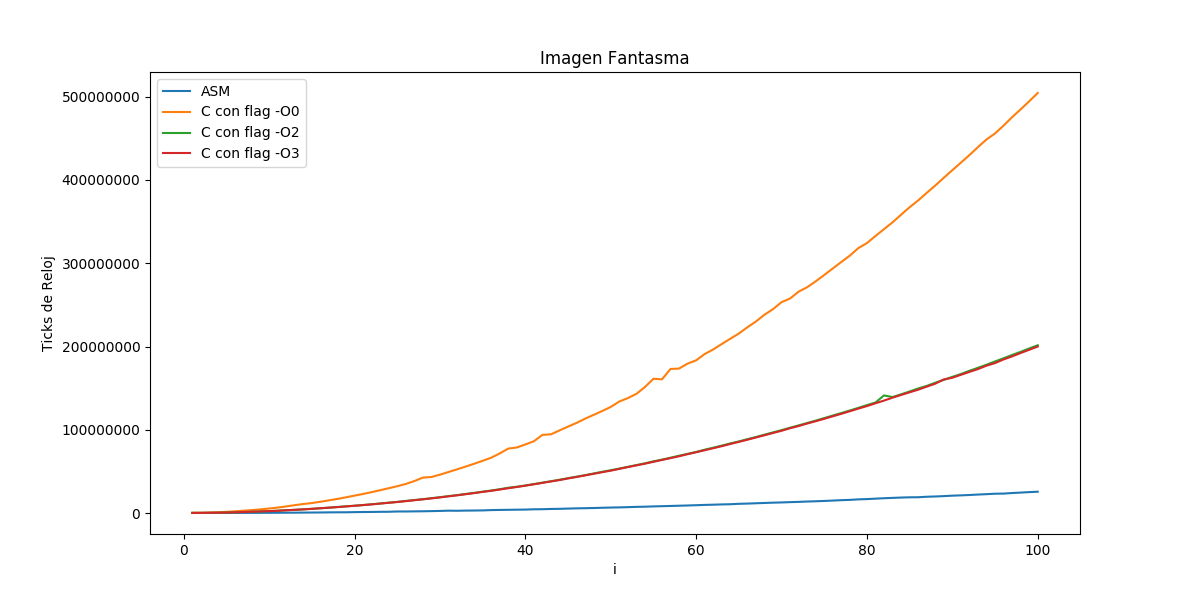
\includegraphics[width=\linewidth]{img/imagenFantasma.png}
			\caption{ImagenFantasma}
			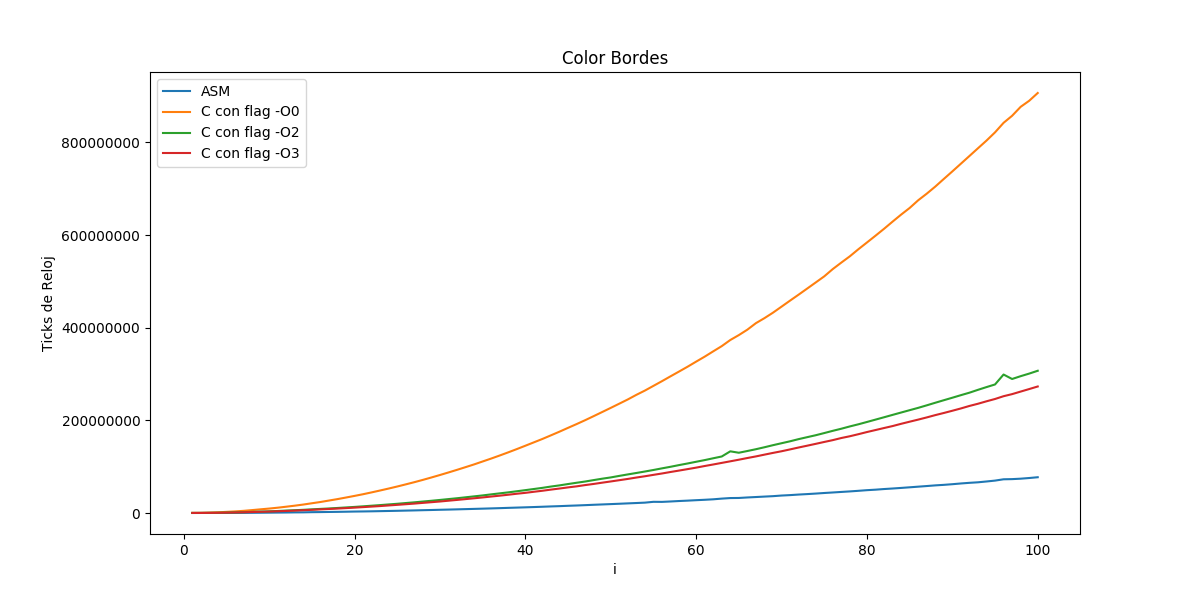
\includegraphics[width=\linewidth]{img/colorBordes.png}
			\caption{Color Bordes}
\end{figure}


\begin{figure}[h!]			
	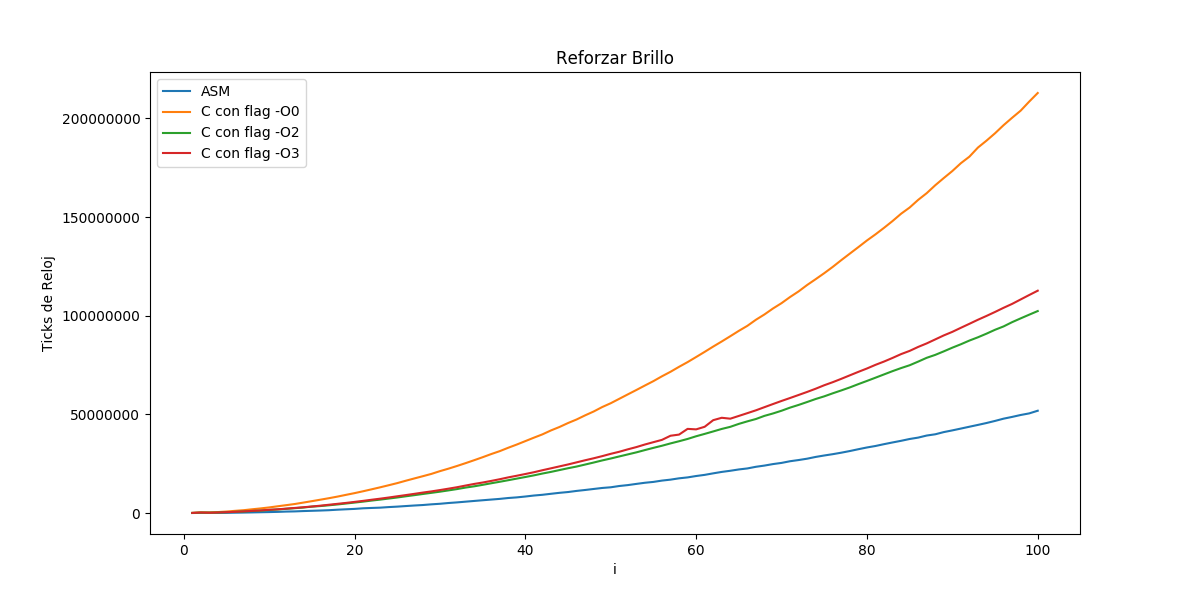
\includegraphics[width=\linewidth]{img/reforzarBrillo.png}
	\caption{Reforzar Brillo}
\end{figure}

\clearpage

\subsubsection{Desenrollado de ciclos}

\begin{figure}[h!]
	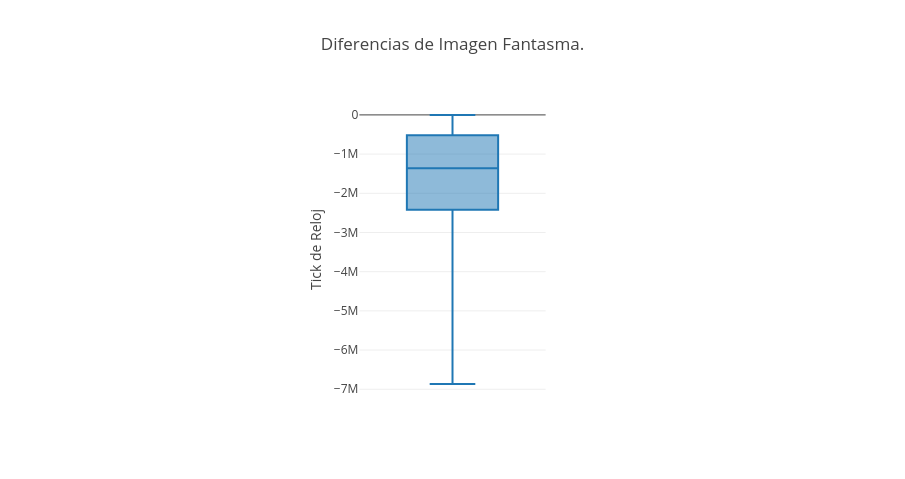
\includegraphics[width=\linewidth]{img/BoxplotImagenFantasma.png}
	\caption{Diferencia de medianas entre Imagen fantasma con ciclos Desenrollados y el filtro original}
\end{figure}

Podemos observar que todos los valores se posicionan por debajo del 0. Los valores dentro del area Q1 y Q3 indican que el desenrollado de ciclos tiende a usar de 500000 a 2,5 millones de ticks de reloj menos, para ponerlo en perspectiva con $i = 100$ el filtro sin modificar usa 25 millones de ticks, esto supone un ahorro del 10\% cuando se desenrollan 10 ciclos. Incluso los valores at\'ipicos fueron a favor del filtro modificado.

\subsubsection{Accesos a memoria}

Como planteamos anteriormente, tomamos las medianas para cada resolución y nos fijamos las diferencias entre la implementación original (A) y la que tiene accesos a memoria en cada iteración (B).


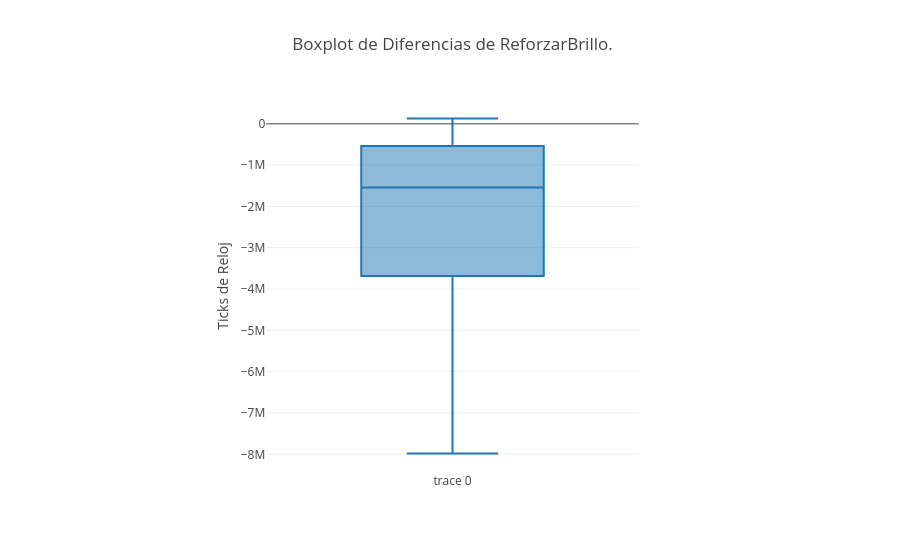
\includegraphics[scale=0.5]{img/BoxplotReforzarBrillo.png}


Como podemos ver en el boxplot de diferencias, la mayoría de valores se encuentra por debajo de 0, lo que quiere decir que la implementaci\'on A corrió mas rápido con respecto a B. En algunos casos B fue efectivamente superior a A. En un vistazo mas cercano buscamos en la tabla de valores estos casos y solo se daban unos pocos con resoluciones muy chicas ($i < 5$). Creemos que al ser resoluciones tan chicas, hay menos misses en la cache ya que logramos recorrer la imagen en menos ciclos.

\section{Conclusiones}
En general pudimos corroborar nuestras hip\'otesis. La implementaci\'on en ASM usando las herramientas de SIMD provee un aprovechamiento de los recursos difícil de alcanzar sin entender el contexto del problema.


\begin{itemize}
	\item Incluso con optimizaciones el código implementado en C era mucho mas lento que nuestra implementación en ASM 
	\item Con el experimento de Desenrollado de ciclos pudimos observar como efectivamente el costo de la predicci\'on de saltos y el overhead de ciclos influye sobre el rendimiento del algoritmo.
	\item Si bien para imágenes muy chicas el acceso a memoria puede no ser tan costoso, sigue siendo un limitante ya que como dijimos en su momento, usar el buffer de memoria puede llegar a condicionar toda la complejidad temporal de nuestro algoritmo.
\end{itemize}

SIMD es una excelente herramienta de bajo nivel para crear algoritmos que trabajan con vectores y matrices de datos, proporcionan un gran rendimiento comparado a implementaciones en lenguajes de alto nivel. Sin embargo este ahorro de complejidad en la ejecución se traspasa a la hora de producir código ya que resulta mucho mas difícil manipular varios datos simultáneamente y aumenta la cantidad de instrucciones.

\end{document}

